\documentclass[12pt,timesnewroman,letterpaper]{article}

%%%%%%%%%%%%%%%%%%%%%%%%%%%%%%%%%%%%%%%%%%%%%%%%%%%%%%%%%%%%%%%%%%%%%%%%%%%%%%%%%%
% Special for e-unibus doc commands

\newcommand{\ForLater}{
\begin{center}
{\bf NOT FOR CURRENT VERSION}
\end{center}
}
\newcommand{\TBC}{\framebox{\textbf{TO BE COMPLETED}}}
\newcommand{\DISCUSS}{\Ovalbox {\bf \textcolor{red}{FOR DISCUSSION}}}
\newcommand{\Input}{\framebox{\textsf{in}}}
\newcommand{\Output}{\framebox{\textsf{out}}}
\newcommand{\debug}[1]{\textbf{debug start} #1 \textbf{debug finish}}
\newcommand{\inx}[1]{\emph{#1}}
\newtheorem{notation}{Notation}
\newtheorem{definition}{Definition}
\newtheorem{problem_statement}{Problem Statement}
\newtheorem{invariant}{Invariant}
\newtheorem{assumption}{Assumption}
\newtheorem{resource_string}{Resource String}
\newtheorem{testcase}{Test Case}
\newtheorem{note}{Note}
\newtheorem{specification}{Specification}
\newtheorem{caution}{Caution}
\newtheorem{prereq}{Pre-requisite}
\newtheorem{action}{Action}
\newtheorem{query}{Query}
\newcommand{\be}{\begin{enumerate}}
\newcommand{\ee}{\end{enumerate}}
\newcommand{\bi}{\begin{itemize}}
\newcommand{\ei}{\end{itemize}}
\newcommand{\bv}{\begin{verbatim}}
\newcommand{\ev}{\end{verbatim}}
\newcommand{\bd}{\begin{description}}
\newcommand{\ed}{\end{description}}
\newcommand{\bpre}{\begin{prereq}}
\newcommand{\epre}{\end{prereq}}
\newcommand{\bact}{\begin{action}}
\newcommand{\eact}{\end{action}}
\newcommand{\bs}{\begin{specification}}
\newcommand{\es}{\end{specification}}
\newcommand{\btc}{\begin{testcase}}
\newcommand{\etc}{\end{testcase}}
\newcommand{\bc}{\begin{caution}}
\newcommand{\ec}{\end{caution}}
\newcommand{\la}{\leftarrow}
\newcommand{\IpArgs}{\subsection{Input Arguments}}
\newcommand{\PreReqs}{\subsection{Pre-requisities}}
\newcommand{\Actions}{\subsection{Actions}}
\newcommand{\Coverage}{{\bf To test coverage.}}

%%%%%%%%%%%%%%%%%%%%%%%%%%%%%%%%%%%%%%%%%%%%%%%%%%%%%%%%%%%%%%%%%%%%%%%%%%%


\newtheorem{theorem}{Theorem}[section]
\newtheorem{lemma}[theorem]{Lemma}
\newtheorem{proposition}[theorem]{Proposition}
\newtheorem{corollary}[theorem]{Corollary}

\newenvironment{proof}[1][Proof]{\begin{trivlist}
\item[\hskip \labelsep {\bfseries #1}]}{\end{trivlist}}
\newenvironment{intuition}[1][Intuition]{\begin{trivlist}
\item[\hskip \labelsep {\bfseries #1}]}{\end{trivlist}}
%% \newenvironment{definition}[1][Definition]{\begin{trivlist}
%% \item[\hskip \labelsep {\bfseries #1}]}{\end{trivlist}}
\newenvironment{example}[1][Example]{\begin{trivlist}
\item[\hskip \labelsep {\bfseries #1}]}{\end{trivlist}}
\newenvironment{remark}[1][Remark]{\begin{trivlist}
\item[\hskip \labelsep {\bfseries #1}]}{\end{trivlist}}

\newcommand{\qed}{\nobreak \ifvmode \relax \else
      \ifdim\lastskip<1.5em \hskip-\lastskip
      \hskip1.5em plus0em minus0.5em \fi \nobreak
      \vrule height0.75em width0.5em depth0.25em\fi}

%%%%%%%%%%%%%%%%%%%%%%%%%%%%%%%%%%%%%%%%%%%%%%%%%%%%%%%%%%%%%%%%%
% \newcommand{\Alogon}{\mbox{\fontfamily{ptm}\selectfont {\large \selectfont A} \hspace{-1.2ex} {\large \selectfont L} \hspace{-2.3ex} \raisebox{0.45ex}{ {\footnotesize \selectfont O} } \hspace{-1.80ex} {\large \selectfont G} \hspace{-1.80ex} \raisebox{-0.33ex}{ {\large \selectfont O} } \hspace{-1.8ex} {\large \selectfont N}}}


\usepackage{times}
\usepackage{mathrsfs}
\usepackage{relsize}
\usepackage{tabto}
\usepackage{amsmath}
\usepackage{helvet}
\usepackage{courier}
\usepackage{fancyheadings}
\pagestyle{fancy}
\usepackage{pmc}
\usepackage{graphicx}
\usepackage{hyperref}
\hypersetup{
    colorlinks=true,
    urlcolor=magenta,
}
\setlength\textwidth{6.5in}
\setlength\textheight{8.5in}
\begin{document}
\title{Logistic Regression in Q}
\author{ Tara Mirmira and Ramesh Subramonian }
\maketitle
\thispagestyle{fancy}
\lfoot{{\small Data Analytics Team}}
\cfoot{}
\rfoot{{\small \thepage}}

\section{Objective}

We have observations that fall into one of two classes: $0$ or $1$. Given a new observation, we want to predict if the observation will be in class $0$ or class $1$. \\

\noindent We would like to use a linear model to make our predictions, meaning we would like to express the class of an observation as a linear combination of the explanatory variables. We consider the simplest linear model, the linear probability model, in the next section.

\section{Linear Probability Model}

Consider the model $y_i = \alpha + \beta x_i + \epsilon_i$


\begin{itemize}
    \item $y_i$ is the class associated with $x_i$, and is what we want to predict
    \item $\epsilon_i$ are independent and identically distributed with mean of $0$ and a variance of $\sigma^2$
    \item $E(y_i) = \alpha + \beta x_i$
    \item $E(y_i) = 0 * P(y_i = 1) + 1*P(y_i = 0) = P(y_i = 1) = \pi_i$
    \item $\pi_i = \alpha + \beta_i$
\end{itemize}

\noindent The problem is $\epsilon_i$ can only take on the values $0$ or $1$ so $Var(\epsilon_i) = (1 - \pi_i)^2 \pi_i + -\pi_i^2(1 - \pi_i) = \pi_i(1-\pi_i)$ which is not constant and non constant variance causes all sorts of problems for linear modelling.\\

\noindent This simple model does not work so we will present a more complex linear model in the next section.

\section{Alternate Model to Linear Probability Model - Linear Model Using Link Function}


General overview:
\begin{itemize}
    \item Let $\pi_i$ be the probability that observation $i$ is in class $1$.
    \item Find a function $G$ such that $\pi_i = G(\alpha + \beta_i)$
    \item We want $G$ to be invertible so we can say $G^{-1}(\pi_i) = \alpha + \beta x_i$
    \item For logistic regression, we will use the function $G(z) = \frac{1}{1+e^{-z}}$
    \item $\frac{1}{1+e^{-z}}$ is bounded between $0$ and $1$ for all values of $z$.
\end{itemize}

\noindent Using the above link function:
\begin{itemize}
    

\item $P(y_i = 1) = \pi_i = G(\alpha + \beta_i) = \dfrac{1}{1 + e^{-(\alpha + \beta x_i)}}  = \dfrac{1}{1 + e^{-(\alpha + \beta x_i)}} * \dfrac{e^{\alpha + \beta x_i}}{e^{\alpha + \beta x_i}} = \dfrac{e^{\alpha + \beta x_i}}{e^{\alpha + \beta x_i} + 1}$
\item $P(y_i = 0) = 1 - P(y_i = 1) = 1 - \dfrac{e^{\alpha + \beta x_i}}{e^{\alpha + \beta x_i} + 1} = \dfrac{1}{1 + e^{\alpha + \beta x_i}}$

\end{itemize}

\noindent \textbf{The odds ratio}: the ratio of the probability of the observation being in one category versus the probability of being in the other category
\begin{itemize}
    
\item odds ratio = $\dfrac{\pi}{1-\pi} = \dfrac{e^{\alpha + \beta x_i}}{1} = e^{\alpha + \beta x_i} = e^{\alpha}e^{\beta x_i}$ which means that when we increase $x_i$ by one unit, the odds increase by $e^{\beta}$

\item $\log(\text{odds ratio}) = \log\big(\dfrac{\pi}{1-\pi}\big) = \log(e^{\alpha + \beta x_i}) = \alpha + \beta x_i$
\end{itemize}

\noindent From the above derivation, we see that we have found the \textbf{link function}:\\\\
$\log\big(\dfrac{\pi_i}{1-\pi_i}\big) = \alpha + \beta x_i$
\\\\
The log of the odds ratio is linear in the ${x_i} 's$. The link function connects $E(y_i) = \pi_i$ to a linear function of the explanatory variables $x_i$.

\section{Fitting a Model to the Data Using Maximum Likelihood}
General overview:
\begin{itemize}
    \item We will use maximum likelihood to estimate $\alpha$ and $\beta$. We want to find $\alpha$ and $\beta$ that makes the given data most likely to occur and use these values to predict future values.
    \item The response variables are the classes $0$ or $1$, which means the response variables are $Bernoulli(\pi_i)$ variables.
\end{itemize}

\noindent Maximum Likelihood:
\\
\\
Recall a few probabilities:
\begin{itemize}
    \item $P(i^{th} \text{ observation } = 1) = \pi_i$
    \item $P(i^{th} \text{ observation } = 0) = 1 - \pi_i$
    \item $P(i^th \text{ observation } = y_i) = \pi_i^{y_i}$ if $y_i = 1$
    \item $P(i^th \text{ observation } = y_i) = (1-\pi_i)^{1-y_i}$ if $y_i = 0$
    \item Using the above two bullet points, $P(i^th \text{ observation } = y_i) =\\ \pi_i^{y_i}(1-\pi_i)^{1-y_i}$
\end{itemize}

$$
\text{Likelihood } = \mathscr{L}(y_1 \ldots y_n) = \prod_{i=1}^{n} p(y_i) = \prod_{i=1}^n P(i^{th} \text{ observation } = y_i) = \prod_{i=1}^n \pi_i^{y_i}(1-\pi_i)^{1-y_i} = 
$$

$$\prod_{i=n}^n \big(\dfrac{\pi_i}{1-\pi_i}\big)^{y_i}(1-\pi_i) = \prod_{i=1}^n (e^{\alpha + \beta x_i})^{y_i}\big(\dfrac{1}{1 + e^{\alpha + \beta x_i}}\big)$$

\noindent Log Likelihood:

$$\log \mathscr{L} = \sum_{i=1}^n y_i(\alpha + \beta x_i) - \log(1 + e^{\alpha + \beta x_i})$$

\noindent We want to find $\alpha$ and $\beta$ that maximize the likelihood of observing the data. To maximize the likelihood (equivalent to maximizing the log likelihood), the next steps are to take the derivatives of the likelihood (or log likelihood) with respect to $\alpha$ and $\beta$, set the equations to $0$, and solve for $\alpha$ and $\beta$.\\\\

\noindent Take the derivative with respect to $\alpha$, set to $0$ and solve:

$$
\dfrac{\partial}{\partial \alpha} \log \mathscr{L} = \sum \big(y_i - \dfrac{1}{1 + e^{\alpha + \beta x_i}}e^{\alpha + \beta x_i}\big) = 0
$$

$$
\sum y_i = \sum \dfrac{e^{\hat{\alpha} + \hat{\beta}x_i}}{1 + e^{\hat{\alpha} + \hat{\beta}x_i}}
$$

\noindent Take the derivative with respect to $\beta$, set to $0$ and solve:

$$
\dfrac{\partial}{\partial \beta} \log \mathscr{L} = \sum \big(y_i x_i - \dfrac{1}{1 + e^{\alpha + \beta x_i}}e^{\alpha + \beta x_i}x_i\big) = 0
$$

$$
\sum y_i x_i = \sum x_i \dfrac{e^{\hat{\alpha} + \hat{\beta} x_i}}{1 + e^{\hat{\alpha} + \hat{\beta} x_i}} \quad \quad (1)
$$

\noindent If we use the design matrix
$$
\boldsymbol{X} = \begin{bmatrix}
    \boldsymbol{1}       & \boldsymbol{x_1} & \dots & \boldsymbol{x_p}
\end{bmatrix}
$$
with $p$ explanatory variables, and the response vector $\boldsymbol{y}$, the equation $(1)$ becomes

$$
\boldsymbol{X^t y} = \boldsymbol{X^t \hat{\pi}}
$$
\\
where $\hat{\pi}$ is the vector of estimated $\pi_i$ values for the observations with values $(1, x_{1,i}, \ldots, x_{p,i})$. $x_{j,i}$ are the observed data values and the $1$ value is added so that an intercept value $\alpha$ is included in the linear model. 
\\\\
This equation is nonlinear so instead of solving directly for $\boldsymbol{\hat{\pi}}$, we will use an iterative method called Newton-Raphson.

\section{Newton-Raphson}

The Newton-Raphson method can be used to approximate the roots of a real-valued function. \\\\
Steps:
\begin{enumerate}
    \item Start with an initial guess $x_0$ for the root
    \item Iterative step: $x_{i+1} = x_i - \dfrac{f(x_i)}{f'(x_i)}$. Note that $(x_{i+1}, 0)$ is the intersection of the $x-axis$ and the line tangent to $f$ at $x_i$
    \item Repeat the iterative step until $f(x_i)$ is sufficiently close to $0$. Then the value $x_i$ is the approximation for the root.
\end{enumerate}

\noindent The diagram at the top of the next page provides a visual for the above steps.\\

\begin{figure}[hbtp]
        \centering
        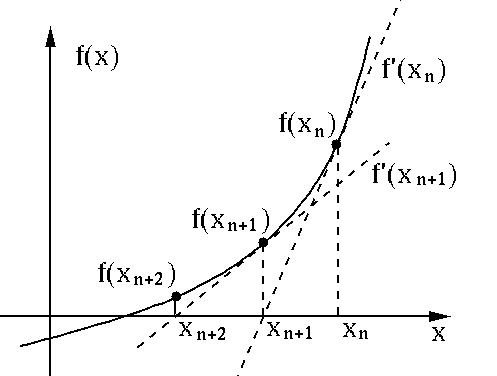
\includegraphics[width=4.5in]{NewtonRaphson.png}
        \caption{Newton Raphson Diagram}
        \label{Newton Raphson}
    \end{figure}

\noindent Next, we will show how to apply the Newton-Raphson method to find the estimate  $\boldsymbol{\hat{\beta}}$ for $\boldsymbol{\beta}$. Note that we have switched to vector notation so instead of estimating $\alpha$ and $\beta$, we want to estimate $\boldsymbol{\beta} = 
\begin{bmatrix} 
    \alpha \\
    \beta_1 \\
    \vdots \\
    \beta_p
\end{bmatrix}$ where $\beta_i$ is the coefficient for the explanatory variable $x_i$ and $\alpha$ is the intercept. \\



\noindent Suppose we want to find the maximum likelihood estimate $\hat{\theta_n}$ for the parameter $\theta$. Let the derivative of the log likelihood function be the function $\ell'$. We want to find the roots of this function, which means we want to find $\hat{\theta_n}$ such that $\ell'(\hat{\theta_n}) = 0$, which means $\hat{\theta_n}$ is the maximum likelihood estimate for $\theta$
\\\\
Recall the general Taylor Series expansion formula:
$$
f(x) = f(a) + \dfrac{f'(a)}{1!}(x - a) + \dfrac{f''(a)}{2!}(x-a)^2 + \ldots
$$
where $f$ is infinitely differentiable at $a$.
\\\\\\
Using a one term Taylor Series expansion, we get that:
$$
\ell'(\hat{\theta_n}) = \ell'(\theta_0) + \ell''(\theta_0)*(\hat{\theta_n} - \theta_0)
$$
\\
It can be shown that $\ell''(\theta_0)$ can be estimated by $E[\ell''(\theta_0)] = -I(\theta_0)$ where $I$ is the Fisher information. \\\\

Now we get:
$$
\ell'(\hat{\theta_n}) = \ell'(\theta_0) - I(\theta_0)*(\hat{\theta_n} - \theta_0)
$$
\\
Rearranging terms we get:
$$
\hat{\theta_n} = \theta_0 + \ell'(\theta_0)[I(\theta_0)]^{-1}
$$

\noindent Now, we can implement Newton-Raphson in the following manner:

\begin{enumerate}
    \item Start with the initial value $\theta_0$
    \item $\theta_{k+1} = \theta_k + \ell'(\theta_k)[I(\theta_k)]^{-1}$
    \item Iterate until $\theta_k \approx \theta_{k+1}$ or until $\ell'(\theta_{k+1}) \approx 0$
\end{enumerate}

\noindent For the case of logistic regression, the parameter $\theta = \boldsymbol{\beta}$\\

\noindent Although not discussed here, it can be shown that for Bernoulli data $I(\boldsymbol{\beta}_{(k)}) = \boldsymbol{X}^t \boldsymbol{W}_{(k)} \boldsymbol{X}$.\\

\noindent $\boldsymbol{W}_{(k)}$ is an $N \times N$ diagonal matrix with the $i^{th}$ diagonal element is $\pi_i(1-\pi_i)$ where $\pi_i$ is the fitted probability for the $i^{th}$ observation using $\boldsymbol{\beta}_{(k)}$\\

\noindent The following is the Newton-Raphson implementation for logistic regression:
\begin{enumerate}
    \item Start with the initial value $\boldsymbol{\beta}_0 = \begin{bmatrix} 
    0 \\
    \vdots \\
    0
    \end{bmatrix}$
    \item $\boldsymbol{\hat{\beta}}_{(k+1)} = \boldsymbol{\hat{\beta}}_{k} + (\boldsymbol{X}^t \boldsymbol{W}_{(k)} \boldsymbol{X})^{-1}[\boldsymbol{X}^t\boldsymbol{y} - \boldsymbol{X}^t\boldsymbol{\hat{\pi}}] = \boldsymbol{\hat{\beta}}_{k} + (\boldsymbol{X}^t \boldsymbol{W}_{(k)} \boldsymbol{X})^{-1}\boldsymbol{X}^t(\boldsymbol{y - \hat{\pi}})$
    \\
    Matrix inversion can be costly. (See \href{https://www.johndcook.com/blog/2010/01/19/dont-invert-that-matrix/}{Don't invert that matrix} for more details). We will manipulate the above equation so the iteration can be performed without needing to invert any matrices.
    \\\\
    $\boldsymbol{\hat{\beta}}_{(k+1)} - \boldsymbol{\hat{\beta}}_{k} = (\boldsymbol{X}^t \boldsymbol{W}_{(k)} \boldsymbol{X})^{-1}\boldsymbol{X}^t(\boldsymbol{y - \hat{\pi}})$
    \\\\
    $(\boldsymbol{X}^t \boldsymbol{W}_{(k)} \boldsymbol{X})(\boldsymbol{\hat{\beta}}_{(k+1)} - \boldsymbol{\hat{\beta}}_{k}) = \boldsymbol{X}^t(\boldsymbol{y - \hat{\pi}})$
    \\\\
    Use a matrix solver to solve for $\boldsymbol{x}$ in $\boldsymbol{Ax} = \boldsymbol{b}$ where 
    \begin{itemize}
    \item $\boldsymbol{A} = \boldsymbol{X}^t \boldsymbol{W}_{(k)} \boldsymbol{X}$
    \item $\boldsymbol{x} = \boldsymbol{\hat{\beta}}_{(k+1)} - \boldsymbol{\hat{\beta}}_{k}$
    \item $\boldsymbol{b} = \boldsymbol{X}^t(\boldsymbol{y - \hat{\pi}})$
    \end{itemize}
    
    Note that $\boldsymbol{\beta}_{(k+1)} = \boldsymbol{x} + \boldsymbol{\hat{\beta}}_{k}$ and $\boldsymbol{\hat{\pi}} = \frac{e^{\boldsymbol{X\beta_{(k)}}}}{1 + e^{\boldsymbol{X\beta_{(k)}}}}$
    
    \item Iterate until $\boldsymbol{\hat{\beta}}$ has converged. At convergence, $(\boldsymbol{X}^t \boldsymbol{W}_{(k)} \boldsymbol{X})^{-1}$ is $\approx 0$
\end{enumerate}

\section{How to Predict the Class of a New Observation}

Recall the link function: 
$$
\log \big( \dfrac{\pi_i}{1-\pi_i} \big) = \alpha + \beta x_i
$$

\noindent We can rewrite this in vector notation as the following:
$$
\log \big( \dfrac{\pi_i}{1-\pi_i} \big) = \boldsymbol{x_i}^t \boldsymbol{\hat{\beta}}
$$

where $\boldsymbol{x_i} = \begin{bmatrix} 
    x_{1,i} \\
    \vdots \\
    x_{p,i}
    \end{bmatrix}$ is the vector that contains the data values for each explanatory variable $x_i$ and $\boldsymbol{\hat{\beta}}$ is the vector of coefficients found by the Newton-Raphson calculation.\\
    
\noindent Given the link function:
$$
\pi_i = \dfrac{e^{\alpha + \beta x_i}}{e^{\alpha + \beta x_i} + 1}
$$

\noindent In vector notation, this is:
$$
\pi_i = \dfrac{e^{\boldsymbol{x_i}^t \boldsymbol{\hat{\beta}}}}{e^{\boldsymbol{x_i}^t \boldsymbol{\hat{\beta}}} + 1}
$$

\noindent Given a new vector of observations $\boldsymbol{z}$, we can plug $\boldsymbol{z}$ in for $\boldsymbol{x_i}$ in the above formula and solve for $\pi_i$. 

A basic classification procedure is the following:

\begin{itemize}
    \item If $\pi_i \geq 0.5$, we classify the new observation as class $1$
    \item If $\pi_i < 0.5$, we classify the new observation as class $0$
\end{itemize}

\noindent The above classification procedure can be modified as desired.


\begin{thebibliography}{9}

\bibitem{notes citation} 
Lecture notes from Professor Deborah Nolan, UC Berkeley, STAT 151A, Spring 2017

\bibitem{stats textbook} 
Trevor Hastie, Robert Tibshirani, and Jerome Friedman. 
\textit{The Elements of Statistical Learning 2nd Edition}. 
Springer, New York, NY, 2009.

\bibitem{image citation} 
Image citation: Ruye Wang - Newton-Raphson method (univariate)
\\\texttt{http://fourier.eng.hmc.edu/e176/lectures/NM/node20.html}

\bibitem{don't invert that matrix}
``Don't invert that matrix" citation: John D. Cook
\\\texttt{https://www.johndcook.com/blog/2010/01/19/dont-invert-that-matrix/}
\end{thebibliography}

\section{Data Structures}

\bi
\item \(X\) is an \(N \times M\) matrix containing the input data concatenated with the value $1$.
  \(X_{i, j}\) is value of \(j^{th}\) attribute of \(i^{th}\)
  instance. \(X\) is stored as \(M\) columns, where \(X_j\) is
  observations for attribute \(j\)

\item \(y\) is an \(N \times 1\) classification vector. \(y_i\) is
  classification of instance \(i\) and can be 1 or 0.
\item \(\beta\) is an \(M \times 1\) coefficient vector. \(\beta_j\)
  is coefficient for attribute \(j\). 
\item \(\beta^{\mathrm new}\) is an \(M \times 1\) vector, which are the new
  coefficients that we solve for in each iteration
\item \(A\) is an \(M \times M\) matrix. Since it is symmetric, we can skip
  computing the lower diagonal elements.
\item \(W = X^TWX\) is a diagonal \(N \times N\) matrix. Since the
  off-diagonal elements are zero, we can represent is as an \(N \times
  1\) vector.   When used as a vector, we will use lower case \(w\). When used
  as a matrix, we will use upper case \(W\). Note that \(W_{i, i} = w_i\) and
  that \( i \neq j \Rightarrow W_{i,j} = 0\)
\item \(b\) is an \(M \times 1\) vector, \(X^T W ( X \beta + W^{-1}(y - p) )\)
  \ei

With these elements, the Newton Raphson iteration becomes the following:
\\
$(X^TWX)\times (\beta^{new} - \beta) = X^T(y-p)$

where 
\be
\item \(W\) is symmetric and positive definite
\item Because \(W\) is symmetric and positive definite, \(A = 
  X^T W X\) is at least positive semi-definite.
\item If the attributes are linearly independent, then \(A\) will actually be
  positive definite; else, the dependent attributes should be removed prior to
  starting the computation.

\framebox{{\bf ANDREW Any easy way to do the above? }}

\ee

\section{computations}

Step by step computations in Table~\ref{step_by_step_calc}.
\begin{table}[ht]
\centering
\begin{tabular}{|l|l|l|l|} \hline \hline
  {\bf Name} & {\bf Description} & {\bf Type} & {\bf Code} \\ \hline \hline
  \(Xbeta\) & \(X \beta\) & \((N \times M) \times (M \times 1)\)  &  \\
  & & \(= N \times 1\) & \(Xbeta = \mathrm{mv\_mul} (X, beta)\) \\ \hline
  \(p\) & & \(N \times 1\) & \( p = \mathrm{logit}(t1) = e^{t1}/(1 + e^{t1})\) \\ \hline
  \(ysubp\) &  \(y - p\) & \(N \times 1\) & \( t_2 = \mathrm{vvsub}(y, p)\) \\ \hline
  \(w\) & & \(N \times 1\) & \( w = \mathrm{logit2}(t1) = e^{t1}/(1 + e^{t1})^2\) \\ \hline
  \(b\) & \(X^T (y-p)\) & \((M\times N) \times (N \times 1)\)
  & \(\forall j_{j=1}^{j=M} b_j = \) \\ 
        & & \( = M \times 1 \) & \(\mathrm{sum}(\mathrm{vvmul}(X_i, ysubp))\) \\ \hline
  \(A\) & \(X^T W X\) & \((M \times N) \times (N \times N) \times (N \times M)\)
  & \(\forall_{j=1}^{j=M} \forall_{k=j}^{k=M} A_{j, k} = \) \\ 
  & & \(= (M \times M)\) & \(\mathrm{sumprod2}(X_j, w, X_k)\) \\ \hline
  \hline

\hline
\end{tabular}
\caption{Listing of individual steps and intermediate values}
\label{step_by_step_calc}
\end{table}

\begin{table}[hb]
\centering
\begin{tabular}{|l|l|l|l|l|} \hline \hline
  {\bf Name} & {\bf Input Type} & {\bf Output Type} & {\bf Return Value} \\ \hline \hline
  logit & Vector \(x\) & Vector \(y\) & \(y = \frac{e^x}{1 + 1^x}\) \\ \hline
  logit2 & Vector \(x\) & Vector \(y\) & \(y = \frac{e^x}{(1 + 1^x)^2}\) \\ \hline
  vvadd & Vector \(x\), Vector \(y\) & Vector \(z\) & \(z = x + y \)  \\ \hline
  vvsub & Vector \(x\), Vector \(y\) & Vector \(z\) & \(z = x - y \)  \\ \hline
  vvmul & Vector \(x\), Vector \(y\) & Vector \(z\) & \(z = x \times y \)  \\ \hline
  vvdiv & Vector \(x\), Vector \(y\) & Vector \(z\) & \(z = x / y \)  \\ \hline
  vsmul & Vector \(x\), Scalar \(y\) & Vector \(z\) & \(\forall i:~z_i = x_ \times y \)  \\ \hline
  sumprod & Vector \(x\), Vector \(y\) & Scalar \(z\) & \(z = \sum_i (x_i \times y_i)\) \\ \hline
  sumprod2 & Vector \(x\), Vector \(y\), Vector \(z\) & Scalar \(w\) &  \(w = \sum_i (x_i \times y_i \times z_i)\) \\ \hline
\hline
\end{tabular}
\caption{Necessary Operators}
\label{tbl_custom_ops}
\end{table}


\section{Details}

\subsection{Notes}

\be
\item The calculation of \(A\) is simplified by the fact that the off-diagonal
  elements of \(w\) are 0 and that it is a symmetric matrix. See last row of
  Table~\ref{step_by_step_calc}
\ee
\subsection{Clarifications needed}

\be
\item Initial guess for \(\beta\)
\ee

\section{Putting it all together}
The Q code will look like the following.

\begin{verbatim}
t1 = mvmul(X, beta)  
p = logit(t1)
w = logit2(t1)
t2 = vvsub(y, p)
for j in 1 to M do 
  b[j] = sumprod(Xj, t2)
end
for j in 1 to M do 
  for k in j to M do 
    A[j][k] = sumprod2(Xj, w, Xk)
  end
end
\end{verbatim}


\end{document}
